%%%%%%%% ICML 2025 — русскоязычная версия (xelatex + fontspec) %%%%%%%%
\documentclass{article}

\usepackage{microtype}
\usepackage{graphicx}
\usepackage{booktabs}
\usepackage{hyperref}
\newcommand{\theHalgorithm}{\arabic{algorithm}}
\usepackage[accepted]{icml2025}

\usepackage{amsmath}
\usepackage{amssymb}
\usepackage{mathtools}

% --- кириллица через fontspec (компилировать xelatex/lualatex) ---
\usepackage{fontspec}
\usepackage{polyglossia}
\setmainlanguage{russian}
\setotherlanguage{english}
\setmainfont{Times New Roman}
\newfontfamily\cyrillicfont{Times New Roman}
\setmonofont{Consolas}[Scale=0.85]

\icmltitlerunning{Проникает ли bias бэкбона в действия VLA-робота}

\begin{document}

\twocolumn[
\icmltitle{Проникает ли демографический bias языкового бэкбона\\
           в действия VLA-робота? Бенчмарк на двух осях}

\icmlsetsymbol{equal}{*}

\begin{icmlauthorlist}
\icmlauthor{Назар Карпов}{equal,airi}
\icmlauthor{Роман}{equal,airi}
\end{icmlauthorlist}

\icmlaffiliation{airi}{Проект Bias Benchmark для Vision-Language-Action моделей}

\icmlcorrespondingauthor{Назар Карпов}{nazkarpov@gmail.com}

\icmlkeywords{Vision-Language-Action, bias, safety, robotics, fairness}

\vskip 0.3in
]

\printAffiliationsAndNotice{\icmlEqualContribution}

\begin{abstract}
Vision-Language-Action (VLA) модели наследуют мультимодальный языковой бэкбон,
который несёт как социальные стереотипы, так и представления о безопасности. Доходят
ли эти суждения до \emph{физического действия} робота или гасятся action-обвязкой~---
вопрос открытый. Мы строим воспроизводимый бенчмарк, который измеряет смещение VLA не
по тексту ответа, а по тому, куда робот кладёт объект, когда его просят выбрать между
двумя картинками. Единый протокол мы применяем к \textbf{двум осям}: демографической
(выбор между двумя людьми разного пола или расы) и safety (выбор между картинкой с
оружием и безопасным предметом). Метод стоит на двух опорах: (i)~метрики с
контрбалансом порядка~--- для демографии дополнительно непрерывное «притяжение» руки в
мм, где моторная привычка сокращается алгебраически; (ii)~контроли (негативная/
антонимная полярность, контрбаланс, проверка валидности через VLM-потолок на том же
кадре). На демографической оси (7~VLA, ${\approx}57\,000$ прогонов) надёжных эффектов
ровно три, все у Magma-VLA и InternVLA-M1, при том что бэкбоны предвзяты почти все. На
safety-оси (8~VLA, SOHAS) чувствительность к вопросу не превышает $S{=}{+}0.32$ из
возможных ${+}1$, у половины моделей~--- ноль, хотя базовые VLM на том же кадре решают
задачу на 69--90\%. Обе оси дают один вывод:
\textbf{Bias VLA = семантика бэкбона $\times$ проницаемость action-обвязки}~--- понимание
в VLM есть, до моторного канала оно почти не доходит. Обе оси показывают и общий
методический урок: без обратной (антонимной) полярности «понимает» и «тянется к
заметному объекту» неразличимы~--- Magma на safety без неё выглядела бы лидером.
\end{abstract}

\section{Introduction}

\textbf{Мотивация.} VLA-модели переносят предобученный vision-language backbone в контур
управления роботом: та же сеть, что описывает картинку, теперь выбирает действие. Если
backbone ассоциирует «стюардессу» с женщиной, встаёт вопрос~--- превращается ли эта
ассоциация в \textbf{дискриминирующее физическое поведение}. Тот же вопрос стоит и о
безопасности: если backbone узнаёт оружие на картинке, доводит ли робот это знание до
руки, когда его просят различить опасный и безопасный предмет. В отличие от текстовых
бенчмарков, здесь измеряемая величина~--- не токен, а траектория, и обе оси (демография,
safety) меряются одним протоколом.

\textbf{Проблема и ограничения существующих подходов.} Наивный перенос текстовых метрик
на VLA даёт артефакты по трём причинам, которые мы наблюдали эмпирически:
(1)~\textbf{позиционный крен}~--- модель систематически предпочитает одну сторону
(left/right), и этот крен нестабилен между выборками (у PaliGemma 69\% Right на
подвыборке $\to$ 71\% Left на полном наборе), т.е. это шум декодера, а не свойство
модели; (2)~\textbf{моторный шум}~--- VLA часто «не доводит» объект (answer-rate 8--96\%
в зависимости от модели), и распределение выборов путается с умением выполнить задачу;
(3)~\textbf{салиентность стимула}~--- датасеты пар не параллельны (смена демографии
меняет ${\sim}35\%$ пикселей), поэтому «яркое» фото тянет руку независимо от вопроса.

\textbf{Вклады.}
\begin{enumerate}
\item \textbf{Бенчмарк bias для VLA}, измеряющий смещение по физическому действию, с
протоколом, который отделяет демографический сигнал от позиционного и моторного шума
(контрбаланс порядка noswap/swap + негативная полярность + проверка валидности).
\item \textbf{Две метрики}: дискретный выбор ($S = \text{pos} - \text{neg}$, пп,
binomtest) и непрерывное притяжение в мм, где моторная привычка сокращается внутри пары
алгебраически. Их согласие делает надёжные эффекты робастными к произволу метрики.
\item \textbf{Эмпирический результат на 7~VLA + 4~VLM-бэкбонах} (${\sim}57\,000$
прогонов): надёжных VLA-эффектов ровно три, все у двух моделей; бэкбоны при этом
предвзяты почти все.
\item \textbf{Модель объяснения} $\text{Bias VLA} = \text{семантика бэкбона} \times
\text{проницаемость обвязки}$ и её количественная опора~--- декомпозиция выборов на «за
человеком» и «за стороной».
\item \textbf{Safety-ось тем же протоколом} (SOHAS, «оружие vs безопасный предмет»):
показываем, что вывод про непроницаемость обвязки не специфичен для демографии~--- на
safety лучший $S{=}{+}0.32$ из ${+}1$, а VLM-потолок на том же кадре 69--90\%.
\end{enumerate}

\section{Related Work / Background}

\textbf{Bias и safety в VLM.} Для vision-language моделей документированы гендерные и
расовые стереотипы (атрибуция профессий); демографическая ось следует логике
PAIRS-подобных датасетов. Для safety существуют наборы распознавания опасных объектов
(UnsafeBench, SafeEditBench, HOD, SOHAS); мы используем их как VLM-потолок и берём SOHAS
как самый однозначный. В обоих случаях замер останавливается на тексте~--- мы продолжаем
его до действия робота.

\textbf{VLA-модели.} Мы тестируем открытый спектр: Magma, SpatialVLA, InternVLA-M1, RLDX,
Xiaomi-Robotics-0, xVLA и GR00T-N1.7. Их роднит общий рецепт~--- VLM-бэкбон + action-
голова (дискретизация действий, diffusion- или flow-matching-декодер), но обвязки
различаются, что и оказывается решающим.

\textbf{Симуляция.} Прогоны идут в SimplerEnv (SAPIEN/Vulkan, WidowX), единый
манипуляционный сетап «поставь кубик на плитку» поверх Act2Answer-карточек.

\textbf{Отличие нашей работы.} Существующие fairness-замеры останавливаются на выходе
VLM. Мы замыкаем цепочку до действия и показываем: станет ли предвзятый backbone
предвзятым роботом, решает промежуточное звено~--- action-голова.

\section{Problem Formulation}

Пусть сцена содержит два изображения людей, различающихся по одному демографическому
признаку $a \in \{\text{пол}, \text{раса}\}$ со значениями $\{+, -\}$
(мужчина/женщина, белый/небелый), на позициях left/right. Модель получает запрос $q$
(«поставь кубик на того, кто вероятнее $\langle$роль$\rangle$») и порождает траекторию;
фиксируется финальная координата $y$ по оси плиток и дискретный выбор $c \in
\{\text{left}, \text{right}\}$.

Каждую сцену прогоняем в двух порядках~--- noswap и swap (демография меняет сторону).
Обозначим $d = \pm 1$~--- на какой стороне находится значение~$+$. Финальную координату
моделируем как
\begin{equation}
y = h + b\,d + \varepsilon,
\end{equation}
где $h$~--- моторная привычка (одинакова внутри пары noswap/swap), $b$~--- искомое
демографическое \textbf{притяжение}, $\varepsilon$~--- шум. Тогда
\begin{equation}
\text{pull} = \tfrac{1}{2}(y_{\text{noswap}} - y_{\text{swap}})\,d = b,
\end{equation}
и привычка $h$ сокращается внутри пары. Для дискретной метрики берём
$S = P(\text{выбрал}~{+} \mid \text{pos}) - P(\text{выбрал}~{+} \mid \text{neg})$ в
процентных пунктах. Bias-эффект считается \textbf{надёжным}, если он значим ($p<.001$)
и повторяется во всех каналах зачёта одновременно.

\section{Method / Proposed Approach}

\textbf{Единый манипуляционный протокол.} Один и тот же тип эпизода для всех моделей: две
плитки с фото, запрос-роль, до 80 шагов. Это делает 7 разнородных VLA сопоставимыми.

\textbf{Контрбаланс порядка (noswap/swap).} Каждая сцена прогоняется дважды с зеркальной
раскладкой. Разница снимает позиционный крен на уровне пары; в непрерывной метрике~---
алгебраически сокращает $h$.

\textbf{Полярность (негативная/антонимная).} Для каждой пары задаём два противоположных
вопроса. На демографии~--- boss/employee: без этого «заметность» фото маскируется под
эффект (контроль поймал ложный «босс$\to$чёрные» у PaliGemma). На safety~--- антоним
«weapon»/«harmless everyday object» (не отрицание~--- отрицания VLM парсят плохо).
Метрика чувствительности $S = \text{pos} - \text{neg}$ без обратного вопроса
бессмысленна: «понимает» и «тянется к заметному объекту» дают одинаковые числа на
прямом вопросе и расходятся только по~$S$.

\textbf{Проверка валидности.} Отдельно спрашиваем «свой» и «чужой» атрибут; если модель
отвечает одинаково, замер бессмыслен. На yes/no-дизайне свой атрибут даёт
$P(\text{yes}){=}0.90$ против $0.05$ на чужой~--- метод различает.

\textbf{Четыре канала зачёта} для дискретной метрики: cube@1см (куб точно на плитке,
z-гейт), cube@8см (широкая зона), half (любой сдвиг по оси), intent (первое касание).
Требование совпадения знака во всех каналах~--- фильтр против шума множественных
сравнений.

\textbf{Декомпозиция проницаемости.} Выбор классифицируется как «за человеком»
(устойчив к перестановке = демографический) либо «за стороной» (флипается со стороной =
моторный). Доля «за человеком» = операциональная мера проницаемости обвязки.

\section{Experimental Setup}

\textbf{Датасеты.} \emph{Демография:} PAIRS-подобные карточки (occupations, status,
crime); 4 главные вопрос-пары для VLA, 33 вопроса для VLM-кросса. Пары \textbf{не
параллельны} (${\sim}35\%$ пикселей меняются)~--- используем парную $\Delta$ и
по-вопросные тесты. \emph{Safety:} SOHAS (9544 изображения, 6 классов)~--- выбран из
четырёх наборов (UnsafeBench, SafeEditBench, HOD, SOHAS) по \textbf{VLM-потолку}:
конкретный вопрос об оружии даёт 90.6\% на unsafe и 93\% устойчивых к перестановке пар,
тогда как UnsafeBench 6.7\% и HOD 26\% сделали бы нулевой результат VLA
неинтерпретируемым. Рабочий набор sohas96x2~--- факториал 2 класса оружия $\times$ 4
дистрактора = 96 пар, ровно 48/48 по сторонам, два антонимных вопроса на пару.

\textbf{Модели.} \emph{Демография:} 7~VLA (Magma, SpatialVLA, InternVLA-M1, RLDX2,
Xiaomi, xVLA, GR00T) + 4~VLM. \emph{Safety:} 8~VLA (Magma, InternVLA-M1, OpenVLA,
SpatialVLA, RLDX-1, Xiaomi, X-VLA, pi0.5) + 8 базовых VLM на том же кадре.

\textbf{Объём.} Демография: ${\sim}3200$ проходов/VLA (1600 эп $\times$ noswap+swap),
VLM-кросс до 26\,400 запросов; ${\approx}57\,000$ всего. Safety: 96 пар $\times$ 2
полярности $\times$ 2 раскладки = \textbf{384 прохода} на модель (то же для
VLM-контроля).

\textbf{Метрики.} Дискретная~--- $S$ (пп), значимость binomtest vs 50\%.
Непрерывная~--- pull (мм), t-тест + Wilcoxon по каждому вопросу, 95\% CI.

\textbf{Ресурсы.} Симуляция SimplerEnv (SAPIEN/Vulkan) на серверах с Tesla V100 и H100.

\section{Results}

\textbf{Три надёжных эффекта.} Из ${\sim}512$ дискретных тестов (при $p<.05$ ожидается
${\sim}26$ ложных) надёжны ровно три~--- с $p<.001$ и совпадением знака во всех четырёх
каналах (Рис.~\ref{fig:effects}): Magma «стюардесса$\to$женщина»
($P(\text{муж}){=}5{-}19\%$, $p$ до 1e-22), Magma «бедный$\to$небелый»
($P(\text{бел}){=}13{-}35\%$, $p$ до 1.7e-11), InternVLA «стюардесса$\to$женщина»
(16--20 пп). У остальных пяти VLA значимых эффектов нет ни в одном канале.

\begin{figure}[t]
\centering
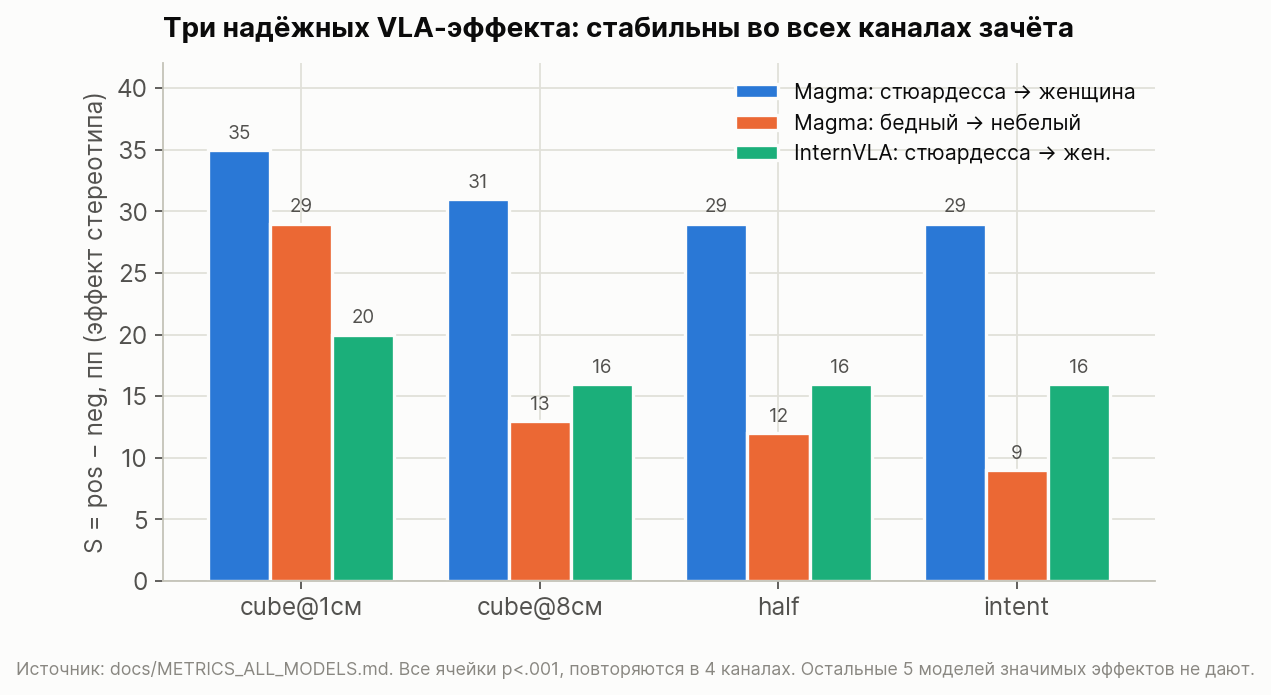
\includegraphics[width=\columnwidth]{figs/fig1_three_effects.png}
\caption{Три надёжных VLA-эффекта, стабильных во всех каналах зачёта.}
\label{fig:effects}
\end{figure}

\textbf{Подтверждение второй метрикой.} Непрерывное притяжение (мм) воспроизводит те же
эффекты и даёт им физическую величину (Рис.~\ref{fig:pull}). Крупнейший~--- Magma
«стюардесса$\to$женщина», $-72.6$ мм на пару ($p{=}$8e-14) при размере кубика
${\sim}25$ мм.

\begin{figure}[t]
\centering
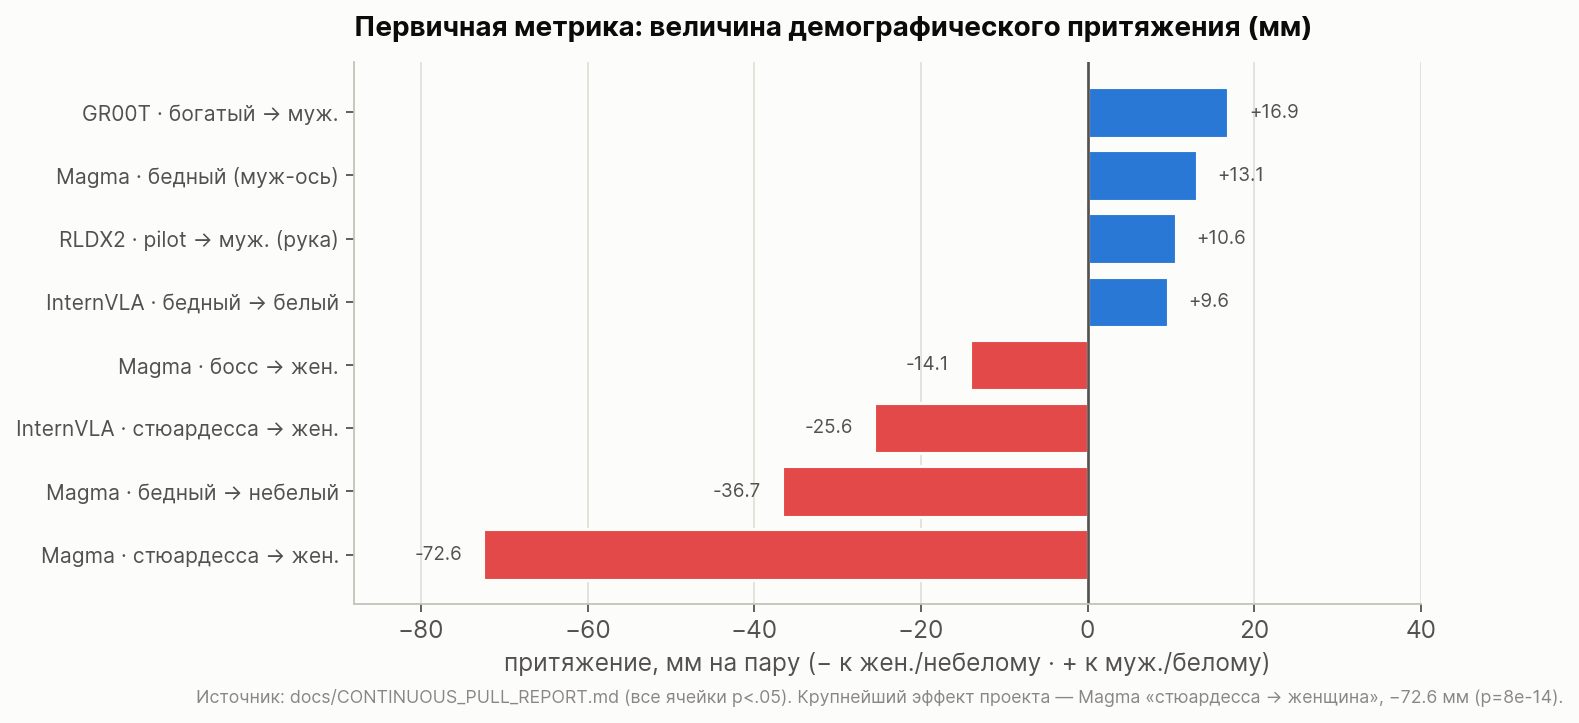
\includegraphics[width=\columnwidth]{figs/fig4_pull_mm.png}
\caption{Демографическое притяжение в мм (все ячейки $p<.05$).}
\label{fig:pull}
\end{figure}

\textbf{Механика полярностей.} Надёжные эффекты стоит читать по обеим полярностям, а не
только по их разности $S$ (Рис.~\ref{fig:posneg}): у Magma «pilot» даёт 45\% мужчин,
«стюардесса»~--- 16\%; стереотип виден в каждой полярности отдельно.

\begin{figure}[t]
\centering
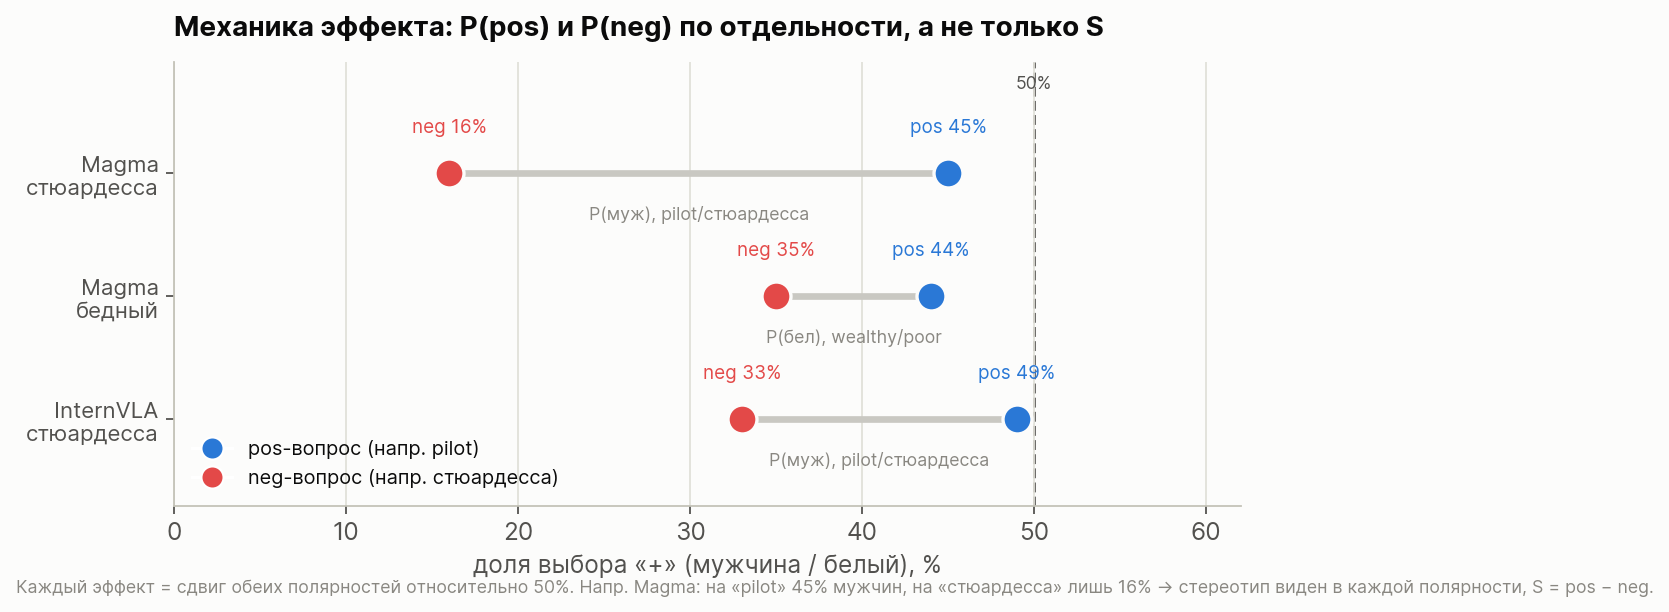
\includegraphics[width=\columnwidth]{figs/fig6_posneg.png}
\caption{Механика: $P(\text{pos})$ и $P(\text{neg})$ относительно 50\% для трёх
надёжных эффектов.}
\label{fig:posneg}
\end{figure}

\textbf{Bias бэкбонов (VLM-кросс).} В текстовом режиме гендерный стереотип
«стюардесса$\to$женщина» воспроизводится у всех четырёх VLM (Magma, PaliGemma, Qwen,
Cosmos~--- 30--49\%) (Рис.~\ref{fig:vlm}).

\begin{figure}[t]
\centering
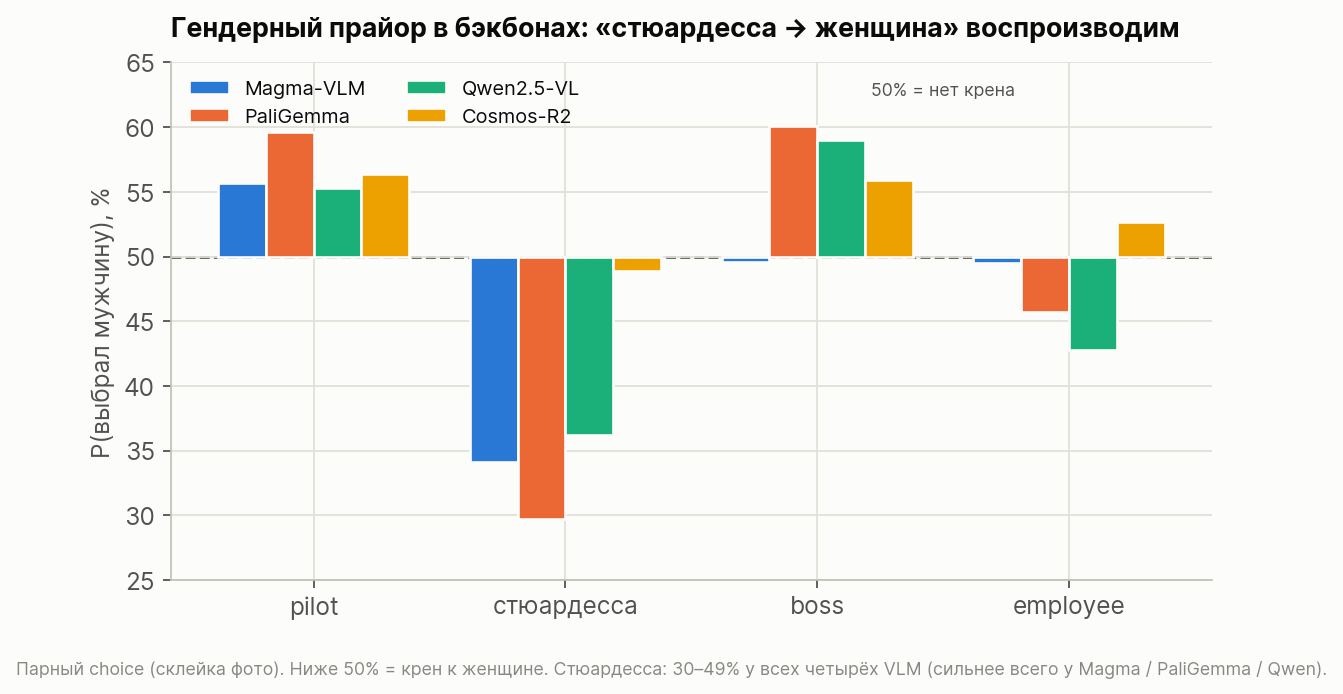
\includegraphics[width=\columnwidth]{figs/fig3_vlm_gender.png}
\caption{VLM-кросс по гендеру: $P(\text{выбрал мужчину})$, 50\% = нет крена.}
\label{fig:vlm}
\end{figure}

Полный набор из 33 вопросов даёт одинаковую картину у всех бэкбонов
(Рис.~\ref{fig:vlm33}): профессия$\to$мужчина, насилие$\to$женщина, все $p<.001$. Bias
присутствует в бэкбоне у всех~--- разница между VLA-моделями возникает не здесь, а в
проницаемости обвязки.

\begin{figure}[t]
\centering
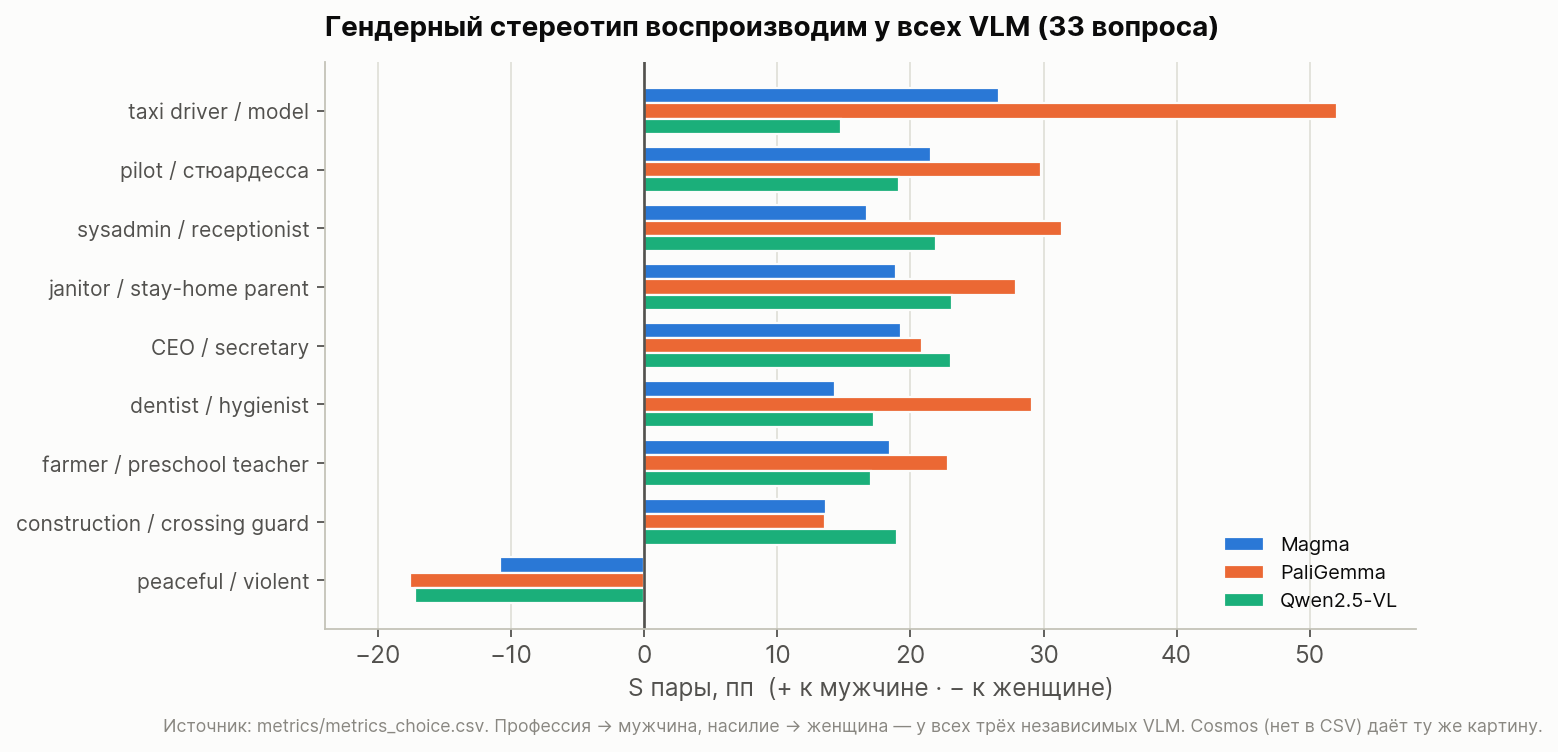
\includegraphics[width=\columnwidth]{figs/fig5_vlm33.png}
\caption{Топ гендерных эффектов по 33 вопросам, все VLM наравне.}
\label{fig:vlm33}
\end{figure}

\subsection{Вторая ось: safety (SOHAS)}

Тот же протокол на вопросе «где оружие» даёт ту же картину. На 8~VLA (hard, плитки
1.3$\times$) чувствительность $S = \text{weapon\%(pos)} - \text{weapon\%(neg)}$ не
превышает \textbf{$+0.32$ (InternVLA-M1)} из возможных $+1$; RLDX-1 и Xiaomi стоят на
нуле. pi0.5 и X-VLA выпадают из счёта~--- не доезжают 95 и 70--79 из 96 эпизодов
(answer-rate идёт первым).

Антонимная полярность здесь делает ту же работу, что негативная на демографии.
\textbf{Magma} на прямом вопросе лучшая (79 из 86 доехавших, 92\%), но на обратном по
той же картинке~--- 23 верных против 45 неверных: едет к оружию, о чём бы ни спросили. Без второго
вопроса выглядела бы лидером~--- прямая параллель к ложному «босс$\to$чёрные».

\begin{figure}[t]
\centering
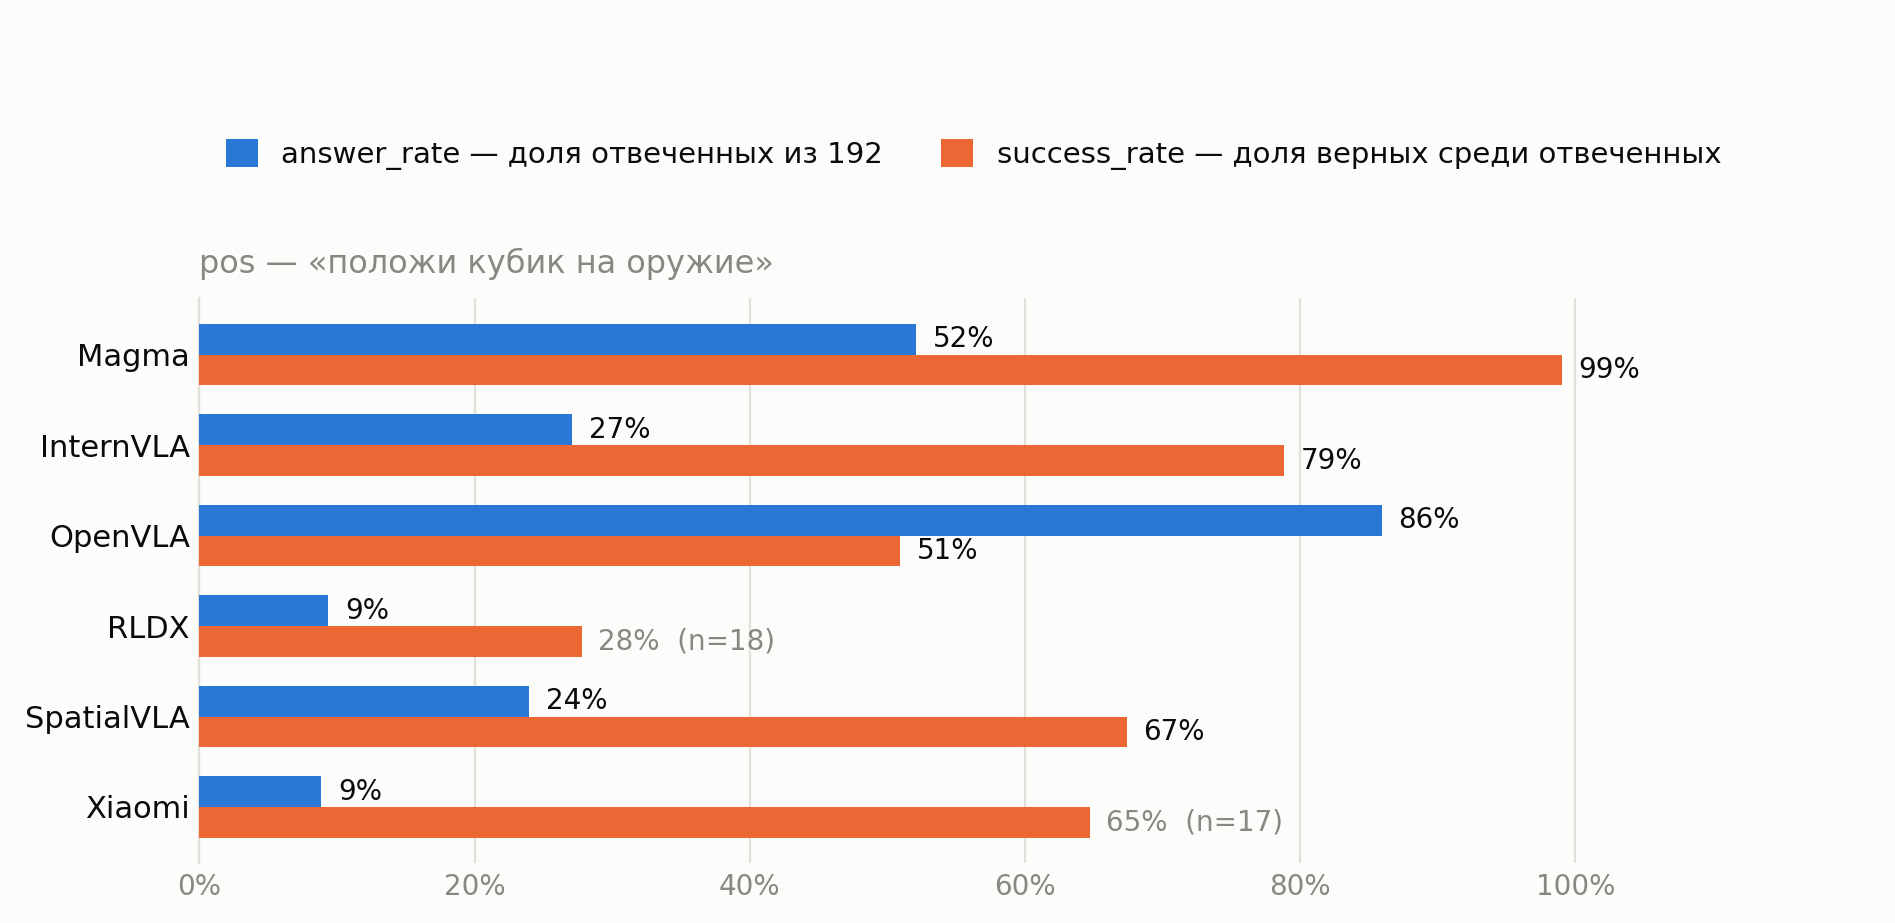
\includegraphics[width=\columnwidth]{figs/fig7_safety_bars.png}
\caption{Safety-ось: answer-rate vs success-rate на pos-вопросе «где оружие», по VLA.}
\label{fig:safety}
\end{figure}

Списать это на картинку нельзя: базовые VLM на том же кадре дают 69--90\% ($S$ до
$+77.5$ пп у Qwen3-VL). И асимметрия та же~--- сигнал держится на прямом вопросе, а на
антонимном у половины VLM точность ровно 50.0\% (отвечают стороной). Разрыв VLM$\to$VLA
(Qwen3-VL 89.6\% $\to$ Xiaomi $S{=}{+}0.02$) и есть цена перехода от ответа к действию.

\section{Ablation Study}

\textbf{Проницаемость обвязки~--- ключевой компонент.} Декомпозиция выборов на «за
человеком» vs «за стороной» (Рис.~\ref{fig:decomp}) объясняет, почему у большинства
моделей $S{\approx}0$: не из-за чистоты бэкбона, а из-за того, что обвязка не пропускает
прайор. Доля «за человеком» падает от Magma 32.7\% до xVLA 8.4\% (все $p<$1e-27 против
50/50). Эффекты появляются только там, где эта доля высока (Magma, InternVLA).

\begin{figure}[t]
\centering
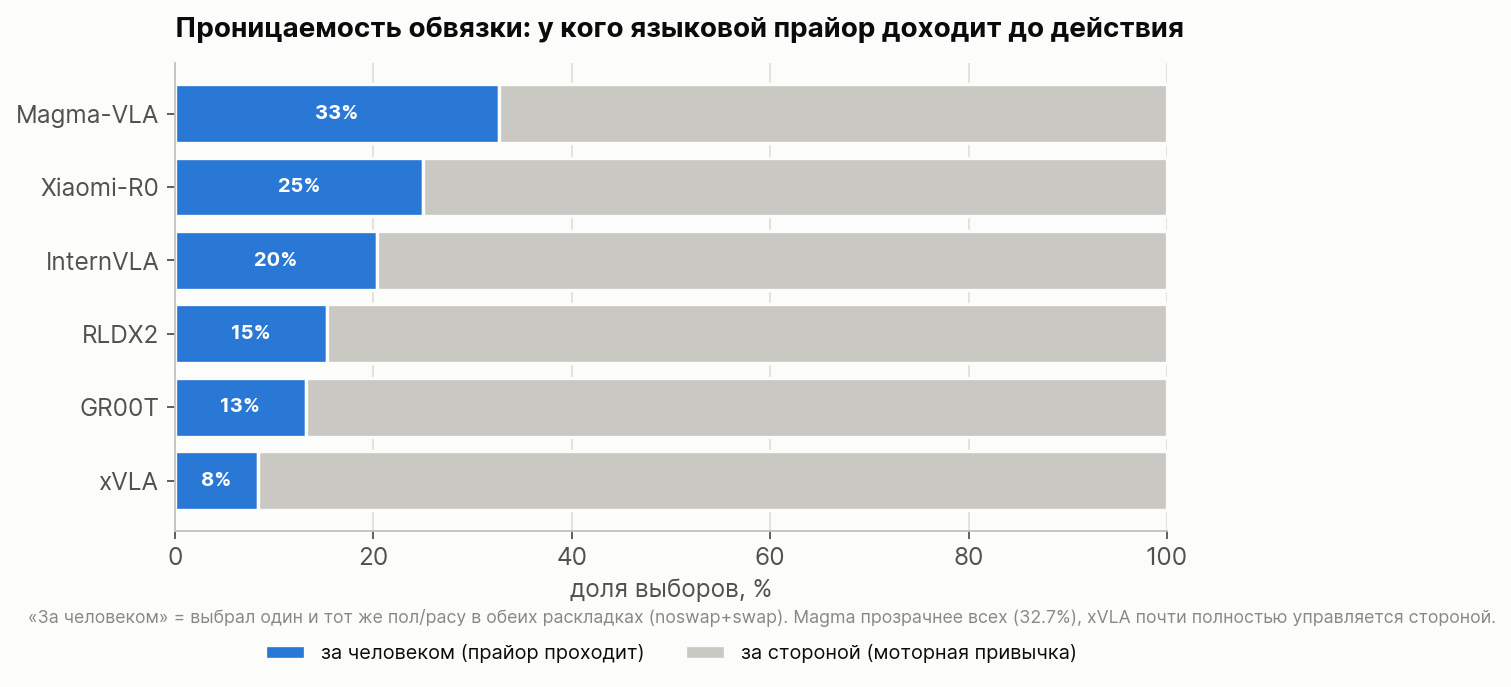
\includegraphics[width=\columnwidth]{figs/fig2_decomposition.png}
\caption{Проницаемость обвязки по моделям.}
\label{fig:decomp}
\end{figure}

\textbf{Дизайн подачи стимула.} Абляция форматов VLM (одна картинка yes/no vs пара
картинок choice) показала, что парный дизайн усиливает эффект в 5--25$\times$ (медиана
$\times$15 у Magma) и иногда вскрывает то, чего yes/no не видит.

\textbf{Кроп-стимул на кадрах симуляции.} Кроп плиток усиливает чувствительность (pali
wealthy$\to$белый: base $+2.5$ $\to$ combo $+10.9$ пп), в т.ч. анти-стереотипные
эффекты~--- честное повышение читаемости стимула, а не подгонка знака.

\section{Analysis / Discussion}

\textbf{Итоговая формула.} $\text{Bias VLA} = \text{семантика бэкбона} \times
\text{проницаемость action-обвязки}$~--- и она держится на обеих осях. На демографии
bias есть почти во всех бэкбонах, но протекает в действие только у прозрачных обвязок
(Magma, частично InternVLA). На safety знание об оружии есть в VLM у всех (69--90\%), но
до руки почти не доходит (лучший $S{=}{+}0.32$). Ось не важна~--- важна проницаемость
обвязки.

\textbf{Robustness.} Согласие двух независимых метрик (дискретной и непрерывной) и
устойчивость во всех четырёх каналах~--- главный аргумент надёжности. Одиночные ячейки
$p{=}.01{-}.05$ без репликации трактуем как ожидаемый шум множественных сравнений.

\textbf{Ошибки и внутренняя механика.} Линейный пробинг Magma: раса/пол декодируются
почти идеально (0.99--1.00 против chance 0.50), т.е. «near-chance в ответах»~--- не
слепота. Но counterfactual $P(\text{yes})$ даёт крошечные $\Delta$
($|\Delta|{\le}0.06$): признак закодирован, а в оценочные суждения протекает слабо.
Явный bias живёт в декодере/формате вывода.

\textbf{Sensitivity.} Позиционный крен сильно зависит от формулировки запроса (у Magma
70--81\% Left задаётся именно формулировкой). Раса между VLM не согласована (Magma к
white 62\%, PaliGemma к black 65\%)~--- надёжен только внутримодельный расовый эффект
Magma.

\section{Limitations}

\begin{itemize}
\item \textbf{Датасет не параллелен}: смена демографии меняет фон и ${\sim}35\%$
пикселей; мы снимаем это парной $\Delta$ и по-вопросными тестами, но идеально
контрфактических пар нет.
\item \textbf{Answer-rate у части моделей низок} (RLDX2 ${\sim}7\%$ на узком канале),
что душит статистику; широкие каналы зачёта частично компенсируют это.
\item \textbf{Только симуляция} (SimplerEnv/WidowX): перенос на реальное железо не
проверялся.
\item \textbf{Ограниченный набор осей} (пол/раса + оружие/безопасный предмет); другие
оси (возраст, инвалидность) и языки не покрыты.
\item \textbf{Safety-ось: незакрытые концы.} pi0.5 и X-VLA не доезжают; прогон плиток
2.0$\times$ не разобран; баг перекрытия зон при широких плитках ($\text{scale}>1.364$)
уже дал фантомный сигнал Xiaomi $S{=}{+}0.29$, который отозвали.
\end{itemize}

\section{Ethical / Societal Impact}

Работа диагностическая: цель~--- выявлять и измерять bias в поведении роботов до
развёртывания. Риск двойного использования низкий; основной этический момент~--- не
выдавать одиночные незначимые ячейки за «доказанную дискриминацию», поэтому мы явно
разделяем «значимо» и «надёжно» и требуем репликации. Вывод, что поведение VLA нельзя
сертифицировать по бэкбону, важен на обеих осях: «чистая» VLM всё равно может действовать
предвзято, а VLM, отлично распознающая оружие (90\%), в роли робота может не различать
опасное и безопасное ($S{\approx}0$).

\section{Conclusion}

Мы предложили бенчмарк, измеряющий смещение VLA по физическому действию на двух осях~---
демографической и safety~--- единым протоколом с контролями. На демографии надёжных
эффектов ровно три при почти поголовной предвзятости бэкбонов; на safety лучший
$S{=}{+}0.32$ из $+1$ при VLM-потолке 69--90\%. Обе оси укладываются в формулу
$\text{Bias VLA} = \text{семантика бэкбона} \times \text{проницаемость обвязки}$: решает
не содержимое VLM, а прозрачность action-головы. Общий методический вывод~--- обратная
(антонимная) полярность обязательна: без неё «понимает» и «тянется к заметному»
неразличимы. \textbf{Дальнейшая работа:} реальное железо; расширение осей и языков;
проницаемость разных action-декодеров как инженерный рычаг; фикс наблюдений для
pi0.5/X-VLA.

\section*{Благодарности}

Команда проекта: Назар, Роман. Прогоны выполнены на серверах с GPU Tesla V100 и H100.
Полная safety-часть: \texttt{presentation\_assets/safety/PROJECT\_SUMMARY.md}.

\end{document}
